            \begin{ledgroupsized}[r]{120mm}
                \footnotesize 
                \pstart                
                \noindent\textbf{\"{U}berlieferung:}   
                \pend
                \end{ledgroupsized}
                            \begin{ledgroupsized}[r]{114mm}
                            \footnotesize 
                            \pstart \parindent -6mm
                            \makebox[6mm][l]{\textit{LiH}}Marginalien und Unterstreichungen im \cite{00163}\textit{Brief Huets an Chouet} vom M\"{a}rz 1673: Leibn. Marg. 105. \pend
                            \end{ledgroupsized}
                %\normalsize
                \vspace*{5mm}
                \begin{ledgroup}
                \footnotesize 
                \pstart
            \noindent\footnotesize{\textbf{Datierungsgr\"{u}nde}: Der Brief tr\"{a}gt das Datum M\"{a}rz 1673}
                \pend
                \end{ledgroup}
            
                \vspace*{8mm}
                \pstart 
                \normalsize
        %  \selectlanguage{french}
           [p.~6] [...] Car, comme celuy-cy ne commence \`{a} jouër, que quand l'eau de sa jambe exterieure a plus de hauteur (son poids estant alors plus grand, l'emporte par dessus l'autre) il arriva de même dans cette experience de l'eau purg\'{e}e\protect\index{Sachverzeichnis}{eau purg\'{e}e}, qu'une petite bulle, qui se forma au bas du col de la phiole, par exemple en A, ne fit que monter le long du col de la phiole, jusques \`{a} ce qu'elle fust parvenuë \`{a} la hauteur d'un pouce au dessus du niveau de l'eau du verre; comme \`{a} la ligne BB, laquelle \'{e}toit un peu au dessus du lieu o\`{u} l'air, rest\'{e} dans le recipient, pouvoit soûtenir l'eau. La colomne AC et la colomne BD avoient jusques l\`{a} combattu par leur poids, [p.~7] comme font toutes les liqueurs; car elles \'{e}toient \'{e}galement press\'{e}es en haut par toute la force de la matiere subtile\protect\index{Sachverzeichnis}{mati\`{e}re!subtile} qui \'{e}toit, d'un cost\'{e}\footnote{\textit{Leibniz unterstreicht}: d'un cost\'{e}} dans la bulle, et de l'autre\footnote{\textit{Leibniz unterstreicht}: de l'autre.\newline%\protect\rule[0cm]{0.5cm}{0cm} 
           \textit{Am Rand auf beide vorausgehenden Unterstreichungen bezogen}: inaequales sunt} dans le recipient; mais comme il ne faut conter la hauteur de la colomne BD que depuis B, puis que ce qui \'{e}toit plus bas \'{e}toit soutenu par l'air, la colomne AC\footnote{\textit{Am Rand}: imo c'est le même avec \textit{ABC}} \'{e}toit toûjours la plus haute; et il faut croire qu'elle l'emportoit par son poids, le matras pourtant ne se vuidoit pas encore pour cela,\footnote{\textit{Am Rand}: non capio} parce qu'il ne pouvoit venir que de l'eau du cost\'{e} de BD, et la bulle cependant montoit, comme font tous les corps plus legers que l'eau.\pend
         \clearpage
         \pstart\selectlanguage{latin}
% Zeitz auskommentiert                 \begin{center}
%          % \begin{wrapfigure}{l}{0.4\textwidth}                    
%                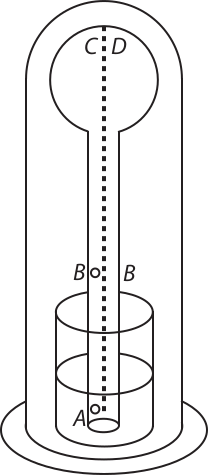
\includegraphics[width=0.3\textwidth]{images/huet}\\\textit{[Fig. 1]}  \footnote{\textit{Zur Zeichnung}: Statim ab initio quando bulla est in \textit{A} major erit pressio ab \textit{A} versus \textit{C} quam a \textit{B} versus \textit{D}, nam illic est materiae subtilis in recipiente et bulla, hic ejus e recipiente tantum. Statim ergo deberet elevare columnam \textit{AB}.} 
%
%                        %\caption{Bildbeschreibung}
%                        \end{center}
                              \edtext{}{\lemma{est}\linenum{|2|||2|}\Afootnote{ \textit{ (1) }\ aeris in reci \textit{ (2) }\ materiae subtilis in recipiente \textit{ L}}}
          \edtext{}{\lemma{hic}\linenum{|3|||3|}\Afootnote{ \textit{ (1) }\ in bulla \textit{ (2) }\ ejus e recipiente \textit{ L}}}
                        %\end{wrapfigure}
                        %@ @ @ Dies ist eine Abstandszeile - fuer den Fall, dass mehrere figures hintereinander kommen, ohne dass dazwischen laengerer Text steht. Dies kann zu einer Fahlermeldung fuehren. @ @ @ \\
                    \pend